\documentclass[border=4pt]{standalone}
\usepackage{tikz}
\usetikzlibrary{arrows.meta, calc, positioning, fit, backgrounds}
\usepackage{amsmath, amssymb}

% Palette shared with fig_interleaved_pipeline.tex
\definecolor{gnnblue}{RGB}{70,130,190}
\definecolor{gnnfill}{RGB}{210,228,248}
\definecolor{bpgreen}{RGB}{60,155,90}
\definecolor{bpfill}{RGB}{210,240,215}
\definecolor{filmorange}{RGB}{210,120,40}
\definecolor{fillfill}{RGB}{252,235,205}
\definecolor{iogray}{RGB}{100,100,100}
\definecolor{iofill}{RGB}{235,235,235}
\definecolor{lossred}{RGB}{190,70,70}
\definecolor{lossfill}{RGB}{250,225,225}

% Matches Table 2 and Secs. 5.3-5.4: training through 10-iteration flooding BP
% on drifting data (p in [0.005, 0.045]) with focal loss on e_z; evaluation on
% separately seeded held-out shots in Regime A (flooding BP) and Regime B
% (serial BP-OSD), each against the same decoder without the GNN.

\begin{document}
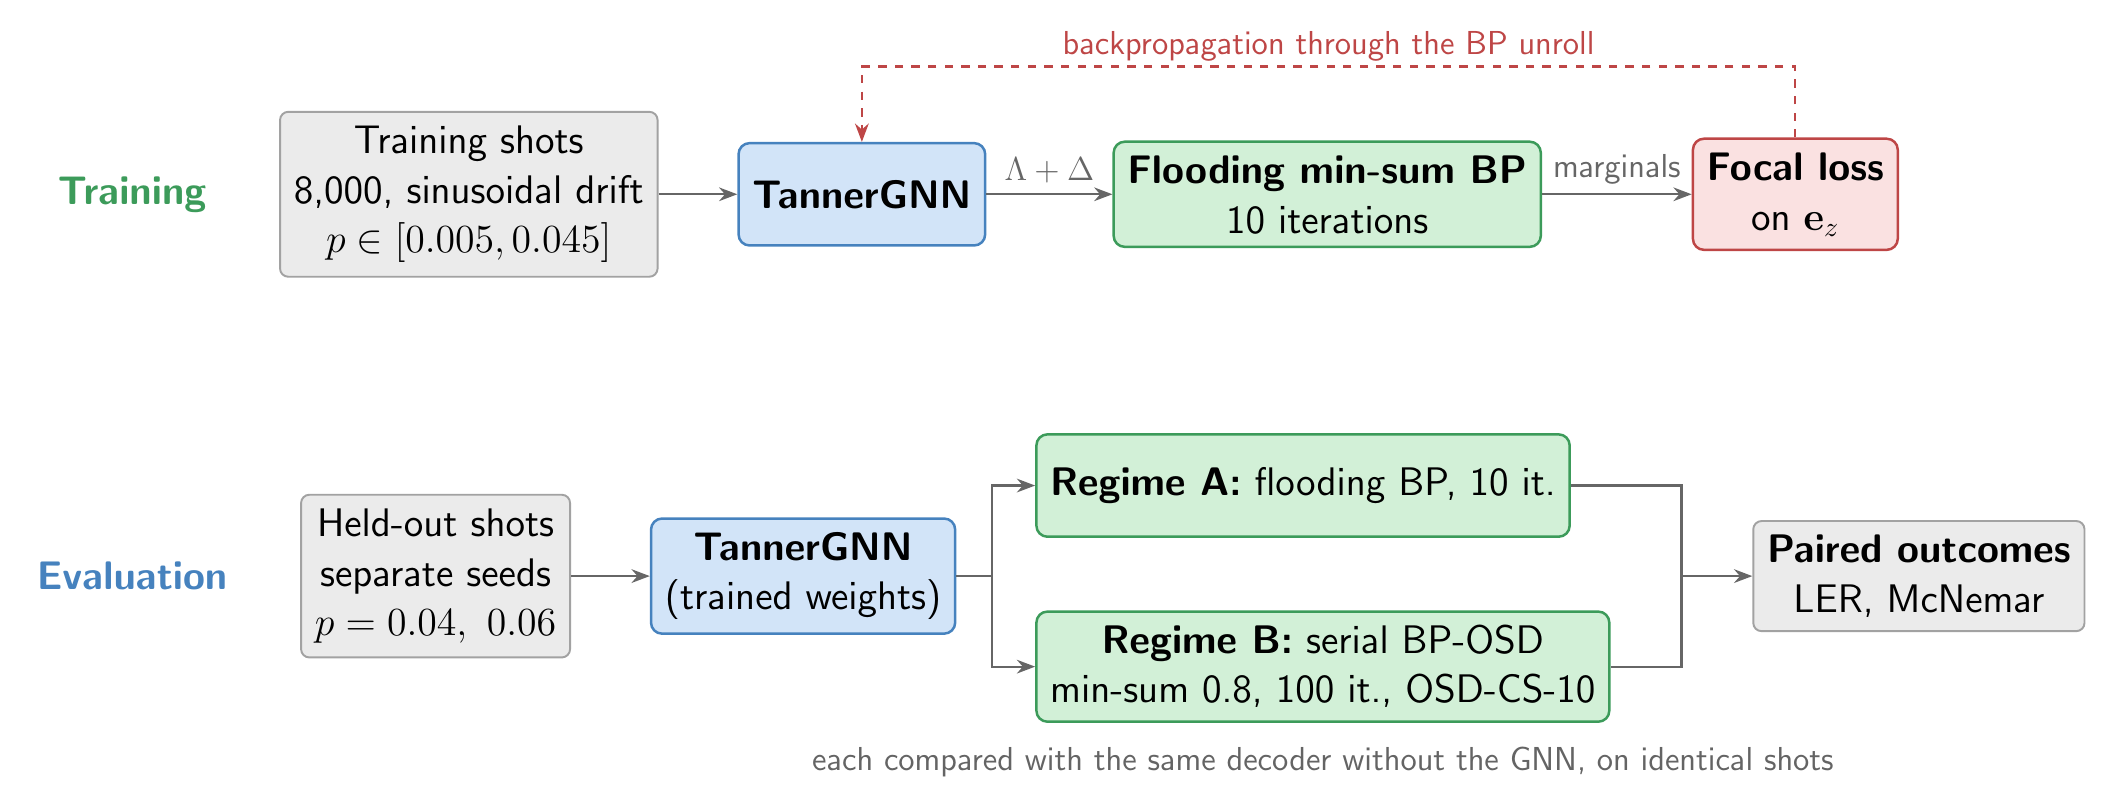
\begin{tikzpicture}[
    >=Stealth,
    font=\sffamily\Large,
    io/.style   = {rectangle, draw=iogray!60, fill=iofill, line width=0.7pt,
                   rounded corners=3pt, align=center, minimum height=1.3cm, inner sep=5pt},
    gnn/.style  = {rectangle, draw=gnnblue, fill=gnnfill, line width=0.9pt,
                   rounded corners=4pt, align=center, minimum height=1.3cm, inner sep=5pt},
    bp/.style   = {rectangle, draw=bpgreen, fill=bpfill, line width=0.9pt,
                   rounded corners=4pt, align=center, minimum height=1.3cm, inner sep=5pt},
    loss/.style = {rectangle, draw=lossred, fill=lossfill, line width=0.9pt,
                   rounded corners=4pt, align=center, minimum height=1.3cm, inner sep=5pt},
    arr/.style  = {->, thick, black!60},
    lane/.style = {font=\sffamily\Large\bfseries, align=center},
    lbl/.style  = {font=\sffamily\large, inner sep=1.5pt},
]

% ---------------- training lane ----------------
\node[lane, text=bpgreen] (tlane) at (0,0) {Training};
\node[io, right=0.8cm of tlane] (tdata) {Training shots\\8{,}000, sinusoidal drift\\$p\in[0.005,0.045]$};
\node[gnn, right=1.0cm of tdata] (tgnn) {\textbf{TannerGNN}};
\node[bp, right=1.6cm of tgnn] (tbp) {\textbf{Flooding min-sum BP}\\10 iterations};
\node[loss, right=1.9cm of tbp] (tloss) {\textbf{Focal loss}\\on $\mathbf{e}_z$};
\draw[arr] (tdata) -- (tgnn);
\draw[arr] (tgnn) -- node[lbl, above=2pt] {$\Lambda+\Delta$} (tbp);
\draw[arr] (tbp) -- node[lbl, above=2pt] {marginals} (tloss);
\draw[arr, dashed, lossred] (tloss.north) -- ++(0,0.9) -| node[lbl, pos=0.25, above, text=lossred] {backpropagation through the BP unroll} (tgnn.north);

% ---------------- evaluation lane ----------------
\node[lane, text=gnnblue, below=4.2cm of tlane] (elane) {Evaluation};
\node[io, right=0.8cm of elane] (edata) {Held-out shots\\separate seeds\\$p=0.04,\ 0.06$};
\node[gnn, right=1.0cm of edata] (egnn) {\textbf{TannerGNN}\\(trained weights)};
\node[bp, right=1.0cm of egnn, yshift=1.15cm] (eA) {\textbf{Regime A:} flooding BP, 10 it.};
\node[bp, right=1.0cm of egnn, yshift=-1.15cm] (eB) {\textbf{Regime B:} serial BP-OSD\\min-sum 0.8, 100 it., OSD-CS-10};
\coordinate (merge) at ($(eB.east |- egnn.east)+(0.9,0)$);
\coordinate (mergeA) at (merge |- eA.east);
\coordinate (mergeB) at (merge |- eB.east);
\node[io, right=0.9cm of merge, anchor=west] (eout) {\textbf{Paired outcomes}\\LER, McNemar};
\draw[arr] (edata) -- (egnn);
\draw[arr] (egnn.east) -- ++(0.45,0) |- (eA.west);
\draw[arr] (egnn.east) -- ++(0.45,0) |- (eB.west);
\draw[thick, black!60] (eA.east) -- (mergeA) -- (mergeB) -- (eB.east);
\draw[arr] (merge) -- (eout.west);
\node[lbl, iogray, below=0.25cm of eB] {each compared with the same decoder without the GNN, on identical shots};

\end{tikzpicture}
\end{document}
